%%%%%%%%%%%%%%%%%%%%%%%%%%%%%%%%%%%%%%%%%
% Lachaise Assignment
% LaTeX Template
% Version 1.0 (26/6/2018)
%
% This template originates from:
% http://www.LaTeXTemplates.com
%
% Authors:
% Marion Lachaise & François Févotte
% Vel (vel@LaTeXTemplates.com)
%
% License:
% CC BY-NC-SA 3.0 (http://creativecommons.org/licenses/by-nc-sa/3.0/)
% 
%%%%%%%%%%%%%%%%%%%%%%%%%%%%%%%%%%%%%%%%%

%----------------------------------------------------------------------------------------
%	PACKAGES AND OTHER DOCUMENT CONFIGURATIONS
%----------------------------------------------------------------------------------------

\documentclass{article}
\usepackage{hyperref}
\usepackage{bm}
\usepackage{booktabs}
\usepackage{titlesec}
 
%%%%%%%%%%%%%%%%%%%%%%%%%%%%%%%%%%%%%%%%%
% Lachaise Assignment
% Structure Specification File
% Version 1.0 (26/6/2018)
%
% This template originates from:
% http://www.LaTeXTemplates.com
%
% Authors:
% Marion Lachaise & François Févotte
% Vel (vel@LaTeXTemplates.com)
%
% License:
% CC BY-NC-SA 3.0 (http://creativecommons.org/licenses/by-nc-sa/3.0/)
% 
%%%%%%%%%%%%%%%%%%%%%%%%%%%%%%%%%%%%%%%%%

%----------------------------------------------------------------------------------------
%	PACKAGES AND OTHER DOCUMENT CONFIGURATIONS
%----------------------------------------------------------------------------------------

\usepackage{amsmath,amsfonts,stmaryrd,amssymb} % Math packages

\usepackage{enumerate} % Custom item numbers for enumerations

\usepackage[ruled]{algorithm2e} % Algorithms

\usepackage[framemethod=tikz]{mdframed} % Allows defining custom boxed/framed environments

\usepackage{listings} % File listings, with syntax highlighting
\lstset{
	basicstyle=\ttfamily, % Typeset listings in monospace font    
	tabsize=4,
}

%----------------------------------------------------------------------------------------
%	DOCUMENT MARGINS
%----------------------------------------------------------------------------------------

\usepackage{geometry} % Required for adjusting page dimensions and margins

\geometry{
	paper=a4paper, % Paper size, change to letterpaper for US letter size
	top=2.5cm, % Top margin
	bottom=3cm, % Bottom margin
	left=2.5cm, % Left margin
	right=2.5cm, % Right margin
	headheight=14pt, % Header height
	footskip=1.5cm, % Space from the bottom margin to the baseline of the footer
	headsep=1.2cm, % Space from the top margin to the baseline of the header
	%showframe, % Uncomment to show how the type block is set on the page
}

%----------------------------------------------------------------------------------------
%	FONTS
%----------------------------------------------------------------------------------------

\usepackage[utf8]{inputenc} % Required for inputting international characters
\usepackage[T1]{fontenc} % Output font encoding for international characters

\usepackage{XCharter} % Use the XCharter fonts

%----------------------------------------------------------------------------------------
%	COMMAND LINE ENVIRONMENT
%----------------------------------------------------------------------------------------

% Usage:
% \begin{commandline}
%	\begin{verbatim}
%		$ ls
%		
%		Applications	Desktop	...
%	\end{verbatim}
% \end{commandline}

\mdfdefinestyle{commandline}{
	leftmargin=10pt,
	rightmargin=10pt,
	innerleftmargin=15pt,
	middlelinecolor=black!50!white,
	middlelinewidth=2pt,
	frametitlerule=false,
	backgroundcolor=black!5!white,
	frametitle={Command Line},
	frametitlefont={\normalfont\sffamily\color{white}\hspace{-1em}},
	frametitlebackgroundcolor=black!50!white,
	nobreak,
}

% Define a custom environment for command-line snapshots
\newenvironment{commandline}{
	\medskip
	\begin{mdframed}[style=commandline]
}{
	\end{mdframed}
	\medskip
}

%----------------------------------------------------------------------------------------
%	FILE CONTENTS ENVIRONMENT
%----------------------------------------------------------------------------------------

% Usage:
% \begin{file}[optional filename, defaults to "File"]
%	File contents, for example, with a listings environment
% \end{file}

\mdfdefinestyle{file}{
	innertopmargin=1.6\baselineskip,
	innerbottommargin=0.8\baselineskip,
	topline=false, bottomline=false,
	leftline=false, rightline=false,
	leftmargin=1cm,
	rightmargin=1cm,
	singleextra={%
		\draw[fill=black!10!white](P)++(0,-1.2em)rectangle(P-|O);
		\node[anchor=north west]
		at(P-|O){\ttfamily\mdfilename};
		%
		\def\l{3em}
		\draw(O-|P)++(-\l,0)--++(\l,\l)--(P)--(P-|O)--(O)--cycle;
		\draw(O-|P)++(-\l,0)--++(0,\l)--++(\l,0);
	},
	nobreak,
}

% Define a custom environment for file contents
\newenvironment{file}[1][File]{ % Set the default filename to "File"
	\medskip
	\newcommand{\mdfilename}{#1}
	\begin{mdframed}[style=file]
}{
	\end{mdframed}
	\medskip
}

%----------------------------------------------------------------------------------------
%	NUMBERED QUESTIONS ENVIRONMENT
%----------------------------------------------------------------------------------------

% Usage:
% \begin{question}[optional title]
%	Question contents
% \end{question}

\mdfdefinestyle{question}{
	innertopmargin=1.2\baselineskip,
	innerbottommargin=0.8\baselineskip,
	roundcorner=5pt,
	nobreak,
	singleextra={%
		\draw(P-|O)node[xshift=1em,anchor=west,fill=white,draw,rounded corners=5pt]{%
		Question \theQuestion\questionTitle};
	},
}

\newcounter{Question} % Stores the current question number that gets iterated with each new question

% Define a custom environment for numbered questions
\newenvironment{question}[1][\unskip]{
	\bigskip
	\stepcounter{Question}
	\newcommand{\questionTitle}{~#1}
	\begin{mdframed}[style=question]
}{
	\end{mdframed}
	\medskip
}

%----------------------------------------------------------------------------------------
%	WARNING TEXT ENVIRONMENT
%----------------------------------------------------------------------------------------

% Usage:
% \begin{warn}[optional title, defaults to "Warning:"]
%	Contents
% \end{warn}

\mdfdefinestyle{warning}{
	topline=false, bottomline=false,
	leftline=false, rightline=false,
	nobreak,
	singleextra={%
		\draw(P-|O)++(-0.5em,0)node(tmp1){};
		\draw(P-|O)++(0.5em,0)node(tmp2){};
		\fill[black,rotate around={45:(P-|O)}](tmp1)rectangle(tmp2);
		\node at(P-|O){\color{white}\scriptsize\bf !};
		\draw[very thick](P-|O)++(0,-1em)--(O);%--(O-|P);
	}
}

% Define a custom environment for warning text
\newenvironment{warn}[1][Warning:]{ % Set the default warning to "Warning:"
	\medskip
	\begin{mdframed}[style=warning]
		\noindent{\textbf{#1}}
}{
	\end{mdframed}
}

%----------------------------------------------------------------------------------------
%	INFORMATION ENVIRONMENT
%----------------------------------------------------------------------------------------

% Usage:
% \begin{info}[optional title, defaults to "Info:"]
% 	contents
% 	\end{info}

\mdfdefinestyle{info}{%
	topline=false, bottomline=false,
	leftline=false, rightline=false,
	nobreak,
	singleextra={%
		\fill[black](P-|O)circle[radius=0.4em];
		\node at(P-|O){\color{white}\scriptsize\bf i};
		\draw[very thick](P-|O)++(0,-0.8em)--(O);%--(O-|P);
	}
}

% Define a custom environment for information
\newenvironment{info}[1][Info:]{ % Set the default title to "Info:"
	\medskip
	\begin{mdframed}[style=info]
		\noindent{\textbf{#1}}
}{
	\end{mdframed}
}
 % Include the file specifying the document structure and custom commands
\setlength{\parskip}{0.2em}

\titlespacing*{\section}
{0pt}{1em}{1em}
\titlespacing*{\subsection}
{0pt}{0.5em}{0.5em}

\def\x{{\mathbf x}}
\def\X{{\mathbf X}}

\def\L{{\cal L}}

%----------------------------------------------------------------------------------------
%	ASSIGNMENT INFORMATION
%----------------------------------------------------------------------------------------

\title{ \large ECS7012P Music and Audio Programming • Spring 2021 \\ \huge Final Project: Zero-latency convolution on Bela} % Title of the assignment

\author{Christian Steinmetz\\ \texttt{c.j.steinmetz@qmul.ac.uk}} % Author name and email address

\date{Queen Mary University of London --- \today} % University, school and/or department name(s) and a date

%----------------------------------------------------------------------------------------

\begin{document}  

\maketitle % Print the title

\section*{Abstract} 

Convolution has many applications in audio, such as equalization and artificial reverberation.
Unfortunately, performing convolution with large filters, as is common in artificial reverberation, 
can be computationally complex when utilizing the direct-form implementation. 
Block-based convolution that takes advantage of the FFT, performing filtering in the frequency domain,
can significantly accelerate this operation, but comes at the cost of higher latency. 
To balance these forces, so-called `zero-latency' convolution has been proposed,
which breaks up the filter so that the early part is implemented with the direct form and later blocks are implemented with the FFT. 
In this project, the goal is to implement a `zero-latency' convolution on the Bela platform to enable real-time effects utilizing large convolutions. 
Furthermore, the ability to utilize this implementation for the creation of a temporal convolutional neural network (TCN) was also investigated. 
While this implementation was able to implement a single large convolution for artificial reverberation,
this alone utilizes a significant portion of the CPU resources on Bela, 
A simple real-time convoluational reverb effect is demonstrated, 
along with a UI that enables users to adjust the quality of the reverb.
Due to the high computational cost of a single convolution, cascading more convolutions in series as is common to implement a TCN was not feasible. 
Future work will incorporate additional optimizations, as well as investigate the applicability of sparsity,
in order to enable large kernel convolutions for the implementation of TCNs in real-time neural audio effects.

\section{Introduction}\label{sec:intro}

The discrete convolution between two signals $x[n]$ and $h[n]$ is given by
\begin{equation*}
    y[n] = \sum_{k=0}^{N-1} h[n] \cdot x[n-k],
\end{equation*}
where $N$ is the number of samples in $h[n]$, often referred to as a filter.
It is common to use $*$ to denote the convolution, 
which can then be written more concisely without the summation as 
\begin{equation*}
    y[n] = x[n] * h[n].
\end{equation*}

Convolution is a foundational operation in signal processing, which has an array of applications. 
From a signal processing perspective, convolution enables the application of finite impulse response (FIR) filters.
These filters are composed of a series of coefficients, which produce an output as a linear combination of the current and past outputs. 
In audio, filtering is one of the predominant use cases, which enables equalization~\cite{valimaki2016all} and artificial reverberation~\cite{valimaki2016more}.
Interestingly, room reverberation can be modeled as an FIR filter given a sufficient number of filter coefficients. 
This entails modeling the room as a linear-time invariant (LTI) system, which is often a reasonable assumption.
The impulse response of the room must be first measured in order to create a filter. 
This process requires both a transducer to generate a signal in the room as well as a receiver to record the resultant sound pressure. 

While early approaches considered impulsive excitation signals, 
like popping a ballon, firing a gun, or simply playing an impulse over a loudspeaker, 
these approaches generally are considered less accurate in capturing the room response. 
This is due to two main reasons. 
First, these excitations signals are often not sufficiently wideband, and therefore exhibit some non-flat frequency response.
This likely colors the resulting room impulse response (RIR) measurement. 
Furthermore, playing an impulse over a loudspeaker is also not ideal due to the nonlinearities of the speaker and amplifier. 
Second, these approaches are also very prone to corruption by environmental noise.
Therefore, common methods for measuring RIRs today generally involve 
either exponential sine sweeps (ESS)~\cite{farina2000simultaneous}, which spread the energy of the impulse out across time, 
as well as the maximum length sequences (MLS), which utilizes multiple noise signals repeated over time~\cite{stan2002comparison}. 

\subsection{Implementation}

Assuming an impulse response of a room has been recorded, the next step in the process is to perform the convolution with an incoming audio signal. 
The common way to implement such an FIR filter is by using what is known as the direct form convolution
\begin{equation*}
    y[n] = h_0 x[n] + h_1 x[n-1] + h_2 x[n-2] + h_3 x[n-3] + \dots + h_{N-1} x[n-N-1]
\end{equation*}
where each output of the filtering process $y[n]$ is computed as given in the previous summation, 
considering a linear combination of past values, with the values of the filter $h_n$ multiplied by the appropriate values. 
This is shown graphically in the block diagram in Figure~\ref{fig:direct}. 
While direct form convolution is quite efficient when the number of coefficients remains small, 
this operation becomes costly as the number of coefficients increases. 
This results in linear scaling, with $O(N)$ multiplies per output point, where $N$ is the number of filter coefficients. 
This is problematic for the application of RIRs where the filter may contain upwards of 
80,000 coefficients for a 2 second long impulse response at a sample rate of 44.1\,kHz. 
This entails over 80,000 multiplies that must occur within a single sampling period, which is 22.6\,$\mu$s.

\begin{figure}
    \centering
    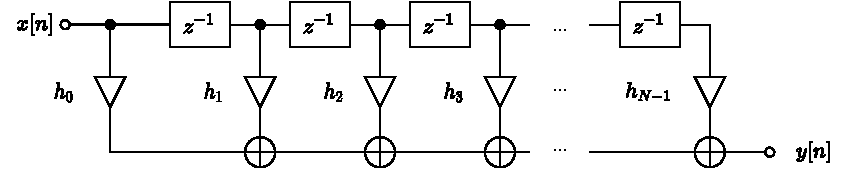
\includegraphics[width=0.7\linewidth]{figures/direct.pdf}
    \caption{Block diagram for the finite impulse response filter implemented with a direct form convolution.}
    \label{fig:direct}
\end{figure}

\subsection{Frequency domain convolution}

This complexity can be reduced by taking advantage of the convolution theorem,
which states that multiplication in the frequency domain is equivalent to convolution in the time domain. 
Therefore, the convolution can be computed by first transforming the input signal and the filter to the frequency domain. 
The complex multiplication (recall that the Fourier transform of a real valued signal is a complex signal) 
of $X[m]$ and $H[m]$ will produce the convolution of the original signals in the frequency domain
\begin{equation*}
    \mathcal{F}\big[ x[n] * h[n] \big] = X[m] \cdot H[m].
\end{equation*}
The time domain output of the convolution can be recovered by taking the inverse fourier transform,
\begin{equation*}
    y[n] =  x[n] * h[n] = \mathcal{F}^{-1}\big[ X[m] \cdot H[m] \big].
\end{equation*}
Applying the filter directly in the frequency domain enables us to take advantage of the fast-Fourier transform (FFT). 
This results in log scaling, with $O(\log N)$ multiplies per output point.
As the number of coefficients in the filter $N$ increases, the frequency domain convolution becomes significantly more efficient than the direct form convolution. 

\begin{figure}
    \centering
    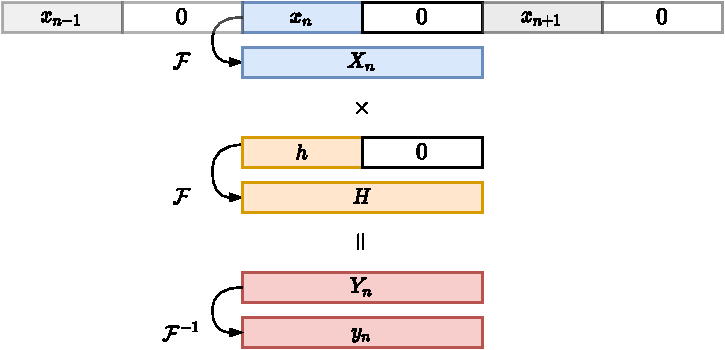
\includegraphics[width=0.7\linewidth]{figures/block-conv.pdf}
    \caption{Block-based FFT convolution between $x_n$ and $h$.}
    \label{fig:block-conv}
\end{figure}

In practice, frequency domain convolution is implemented with a block convolver, as shown in Figure~\ref{fig:block-conv}.
In order to avoid time aliasaing, i.e. to capture the resultant ringing of the convolution between the filter and the input signal, 
an FFT size twice as large of the input blocks is utilized, padding the second half of the time domain input with zeros. 
The frequency domain representation of the filter block $H$ is computed using the FFT, along with incoming blocks of $x[n]$ of equal size.
After complex multiplication in the frequency domain,
the IFFT is performed on the result to produce the time domain output of the filter, $y[n]$. 
In practice, the impulse response is often very large and therefore it is commonly split into smaller 
blocks, often a power of 2 in length ($N \in$ 32, 64, ... 512, ...). 
An overlap-add or overlap-save method can then be used to accumulate the outputs from the convolution with each block, 
adding the filtered signal at the proper offset within the output signal.

\subsection{Low-latency convolution}

While frequency domain convolution achieves superior efficiency as compared to the direct form convolution with larger filters (often $N > 128$),
it imparts a minimum latency of $N$ samples, given by the FFT block size. 
This is due to the fact that $N$ samples must first be accumulated from $x[n]$ before performing the computation. 
This contrasts with direct form convolution which requires only a single input sample to produce the next output, 
but requires significantly more computation when the filter is large. 

Approaches that balance these two forces to achieve computational efficiency and achieve low latency have been proposed~\cite{gardner1994efficient, muller1999low, hurchalla2010time, wefers2015partitioned}.
The implementation in this work focuses on the one proposed by Gardner~\cite{gardner1994efficient}, 
which is also referred to as the `zero-latency' convolution.
While signal processing is never completely free of latency since some time is required in the hardware, 
in this case a 'zero-latency' convolution is an operation wherein the only delay imparted by the system is that of carrying out the computation.
This is another way of saying that no time is needed to `wait around', while samples accumulate in a buffer, imparting latency as they do in the block-based convolution. 

In order to reduce latency while reducing the computation complexity of the convolution, 
this approach utilizes a combination of the direct form and frequency domain convolution implementations. 
As in the block-based frequency domain convolution, the impulse response is broken into separate blocks. 
To achieve the optimal latency and computation tradeoff these impulse response is split into blocks given the pattern in Figure~\ref{fig:blocks}.
The size of the first block $h_0$ is set to $2N$ samples, where N is selected as the block size where the FFT convolution becomes more efficient than the direct form convolution. 
Then $h_1$ and $h_2$ are of size $N$, followed by two blocks of size $2N$, and so on.
The first block is implemented with a direct form convolution immediately in the main processing loop. 
Since the size of this block is selected to be sufficiently small there will be no problem in computing the output within time. 
Then, separate tasks are scheduled to compute the following larger blocks when enough input samples have been collected. 
These tasks are scheduled with decreasing priority, such that the smallest blocks will always be computed with a higher priority 
since they are needed more rapidly than larger blocks. 

\begin{figure}[h]
    \centering
    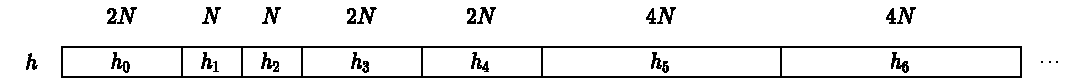
\includegraphics[width=\linewidth]{figures/blocks.pdf}
    \caption{Splitting the impulse response in blocks.}
    \label{fig:blocks}
\end{figure}

\section{Convolutional neural networks}\label{sec:conv}

Changing gears, convolution has found utility in modern deep learning. 
The convolutional neural network (CNN)~\cite{lecun1998gradient} has been of significant interest since
the success of AlexNet~\cite{krizhevsky2012imagenet} in 2012, 
which outperformed previous image classification models by a significant margin.
These neural network architectures are conceptually quite simple,
but a multitude of architectural variations have been investigated.
Nevertheless, the general design consists of a convolution operation, 
followed by downsampling, and then a nonlinear activation function. 

Unlike RIRs, most CNNs in computer vision utilize very small filters. 
This is often $3 \times 3$, $5 \times 5$, or $7 \times 7$ filters. 
While these filters have very limited receptive field, 
they gain larger context by cascading many convolution operations in series, 
with interleaved downsampling operations.
This achieves and effectively large filter by composing many small filters, 
which are efficient to implement using the direct form convolution. 
While there has been some interest in the applicability of FFT-based convolution 
to accelerate these networks~\cite{vasilyev2015cnn, lavin2016fast, abtahi2017accelerating, abtahi2018accelerating}, 
this technique has not seen widespread adoption 
due to the somewhat limited gains when using such small filters. 

\subsection{Temporal convolutional networks}

While there has been significant interest in 2D CNNs both in computer vision as well as in audio, operating on spectral representations,
the temporal convolutional network (TCN)~\cite{bai2018tcn} has seen growing interest in end-to-end audio processing architectures~\cite{rethage2018wavenet}.
First popularized for audio by WaveNet~\cite{oord2016wavenet}, these architectures operate on waveform using a series of dilated 1-D convolutions. 
Since achieving sufficient receptive field with small filters at audio samples rates is not feasible by adding simply additional layers, 
dilated convolutions have become a popular technique for achieving large receptive fields efficiently. 
Dilated convolutions take a small convolutional filter and increase its effective size by inserting zeros within the filter. 
A larger dilation factor inserts more zeros between values of this filter. 
Since the multiplication between the input and any of the zeroed values in the filter will also be zero, these computations can be ignored. 
This provides a high computational cost savings via sparsity as compared to a dense filter of comparable size. 
Interestingly, this approach of very sparse filters have brought acceptable performance.

\subsection{Efficient temporal convolutional networks}

Independent of dilations, one of the easiest ways to increase the efficiency of TCNs is to reduce the number of layers, 
since these computations must occur in series. 
However, reducing the depth of the network significantly reduces the receptive field, which is critical for performance. 
Even when utilizing dilated convolutions as is standard in TCNs, where the dilation factor grows as a function of the depth, 
given by $d_n = 2^n$, where $n \in 1, 2, ..., N$ for an $N$-layer network, 20 to 30 layers are often required.
This present a computational load that restricts real-time performance on CPU.

In contrast, utilizing fewer layers with larger kernels is one route to reducing the computational load~\cite{steinmetz2021efficient}.
This comes at the cost of increased sparsity in the convolutions, yet can enable real-time operation on CPU. 
Another potential route to address this could be the use of very few layers, potentially as little as two, 
which utilize very large filters, and are implemented using a block-based FFT convolution. 
This enables significant receptive field, and could potentially see significant benefit from 
FFT convolution, whereas previous FFT based approaches for small filters have been less impressive. 
While block-based convolutions significantly reduce the computational cost,
as introduced previously, the block size imparts a lowerbound on the latency of the system. 
While this is not often of significant concern in computer vision applications, 
the ability for not only efficient, but also low-latency operation, is critical in real-time audio effects. 

For that reason, there is the potential to first train a TCN that uses very large filters, but few layers, 
using a standard large block size FFT convolution. 
This will provide the most computationally efficient operation when latency is of no concern. 
However, it will also be possible to use a different convolution implementation during inference as compared to training. 
Treating the weights of the convolutional layers in the pre-trained network as large filters means that the 
previously proposed low-latency convolution could be used to implement the neural network.
This is partly the motivation for the investigations presented in this project. 

\section{Design}

As introduced in Section~\ref{sec:intro}, the design of the zero-latency convolution implementation is based heavily on the system proposed by Gardner~\cite{gardner1994efficient}.
In this configuration, the impulse response $h$ is split into a number of blocks of increasing size, as shown in Figure~\ref{fig:blocks}. 
To implement this in code, three classes were designed. 
There are two lower level classes, \texttt{DirectConvolver} and \texttt{FFTConvolver}, 
which implement an isolated direct form convolution and block-based FFT convolution respectively. 
Each of these classes access an external input and output circular buffer in order to read current and past values, 
and then write filtered values to the appropriate place in memory. 
Instances of these classes are instantiated in the higher level \texttt{ZLConvolver} class, 
which implements a complete zero-latency convolution. 

The \texttt{DirectConvolver} class is the simplest. 
During initialization, this class requires a vector containing the coefficients of the filter, 
along with the index of this filter block within the full filter. 
For all practical cases this index is 0, since the direct convolver is generally used to process the first block of the filter. 
At initialization pointers to vectors containing the input and output circular buffer are also required. 
These pointers will be used during the processing phase in order read and write the appropriate data, 
and will be shared among all of the convolvers in the system.

In order to operate the convolver the \texttt{process()} method is called, 
passing a index to the current position to read from within the circular buffer.
Then a single output value will be computed by iterating over the filter coefficients, stored in memory, 
accumulating the value as a function of the current and past output values. 
Finally, this single value is written to the correct position within the output circular buffer, 
and the output write pointer is incremented by a single step. 

The \texttt{FFTConvolver} is somewhat more complex than the direct convolver, but shares many of the same design elements. 
During initialization this class also requires a vector containing the filter coefficients, the offset in the complete filter, 
and pointers to the input and output circular buffer. 
In addition, the FFT size must be provided and it must always be twice as large as the number of samples in the supplied filter. 
In \texttt{setup()} the Bela \texttt{Fft} objects are instantiated for both the current input block \texttt{fftX}, 
the associated filter block \texttt{fftH}, along with a FFT buffer \texttt{fftBuffer} for storing the results of the complex multiplication.
After setting the FFT size for these objects, the values from the provided vector of filter coefficients is loaded into the 
time domain attribute of the \texttt{fftH} object, and the FFT is precomputed.

The process of launching the FFT convolver is somewhat more complicated since it is designed such that it can operate on its own thread. 
The convolver must first be queued by passing an index of where to read from the input circular buffer. 
This index corresponds to the most recent value read into the buffer, and the convolver will read backwards 
up to one half the FFT size. 
After being queued, the \texttt{process()} method must be called to begin the process. 
This is designed so that the main thread in \texttt{render()} can queue the convolver with the correct read pointer, 
but the process will not be launched until there is time, which will be explained in more detail in the following paragraph. 
Within \texttt{process()}, values from the input buffer will be read for the computation, up to one half the FFT size. 
The remaining values for the input block will be zeroes. Then the FFT of the input block will be computed. 
To apply the filter, complex multiplication must be carried out between the frequency domain representations. 
This can be achieved very simply. 
Consider two complex numbers $a + bi$ and $c + di$. 
Their produce can be computed in a similar manner as if these were binomials. 
\begin{align*}
    (a + bi) \cdot (c + di) \\
    ac + (ad)i + (bc)i + (bd)i^2 \\
    ac + (ad + bc)i - (bd) \\
    (ac - bd) + (ad + bc)i
\end{align*}
After the complex multiplication, the IFFT is computed, 
which produces the same number of output samples as the FFT size. 
These values are then written to the appropriate place in the output buffer. 
Since the initial output write index was initialized as the offset of this block within complete filter, 
the output samples should be written to the appropriate location .
As is the usual, modulo arithmetic is utilized to ensure that indices in the circular buffers are wrapped around. 
The final step involves incrementing the write index. 
Even though the convolution will produce FFT size number of samples, 
the write index is only advanced by one half of the FFT size, since this was the number of samples from the input block. 

The \texttt{ZLConvolver} class encapsulates the convolver objects to create an entire convolution system. 
This class is significantly more complex than the lower level classes, and requires managing multiple threads
to run individual processes for each of the \texttt{FFTConvolver} objects.
During initialization the most important parameter is a path to the appropriate wav file from which to load the impulse response. 
The provided \texttt{MonoFilePlayer} class is then utilized to read this data from disk.
The most important step during this process is that of splitting the complete impulse response into a set of blocks, each with their own convolver. 
The original pattern from Figure~\ref{fig:blocks} is followed, where the FFT size is always twice the block size. 
After reading the appropriate number of samples from file player, a new convolver is created for that block. 
Only one \texttt{DirectConvolver} is created for the first block, while \texttt{FFTConvolver} objects are stored in a vector for the remaining blocks. 
The final step during initialization is the creation of a unique thread for each of the \texttt{FFTConvolver} objects.
This is achieved with \texttt{Bela\_createAuxiliaryTask}, storing the resulting task in a vector. 
In order to access the correct convolver, each task passes a pointer to the convolver instance as an argument. 

Along with the convolvers, the \texttt{ZLConvolver} class also maintains the input and output circular buffers. 
When calling the \texttt{process()} method, the next input sample is written into the input buffer. 
Next the \texttt{DirectConvolver} is called to produce the result of this filter block. 
After this, all of the \texttt{FFTConvolvers} are iterated over in order to determine if enough samples 
have accumulated for them to begin processing the next block. 
To facilitate this, the \texttt{convolverBufferSamples\_} vector contains the number of samples 
that have been read since the last time each convolver was run. 
If the value in a position of this vector is equal to one half the FFT size of the respective convolver, 
then this convolver task is launched from the \texttt{convolverThreads\_} array. 
Each convolver task is created with a priority based on the FFT size.
Smaller blocks have a higher priority since they occur more rapidly, while larger blocks are needed less frequently. 
It was found that due to the tight timing constraints, without using these priority values it was not possible to achieve smooth performance.

Following the launching of the convolvers, 
the next value from the output buffer is read, so that it can be written to the audio output on Bela for the current frame. 
This value is then set to 0 in the output circular buffer for the next time it is utilized. 
As a final step the output read pointer is incremented for the next sample. 
Before passing the output sample to the audio output, a wet/dry mix is applied, along with an optional tanh nonlinearity. 

\emph{Note: As a starting point, the design of the code was based upon the code in Lecture 20: Phase vocoder.}

\subsection{Optimizations}

Gardner~\cite{gardner1994efficient} lists a number of optimizations including:

\begin{enumerate}
    \item Precomputing the spectra for all blocks of the filter $h$. 
    \item Utilize real valued FFT to exploit symmetry. 
    \item Expoloit symmetry in the complex multiplication. 
    \item Reuse input spectra from $x$ whenever possible. 
    \item Reuse input spectra from small blocks for large block computations.
\end{enumerate}

In this implementation the first three optimizations are considered. 
The final two optimizations are likely to further improve performance, 
but will require more significant rework of the \texttt{FFTConvolver} class.

\subsection{User interface}

\begin{figure}
    \centering
    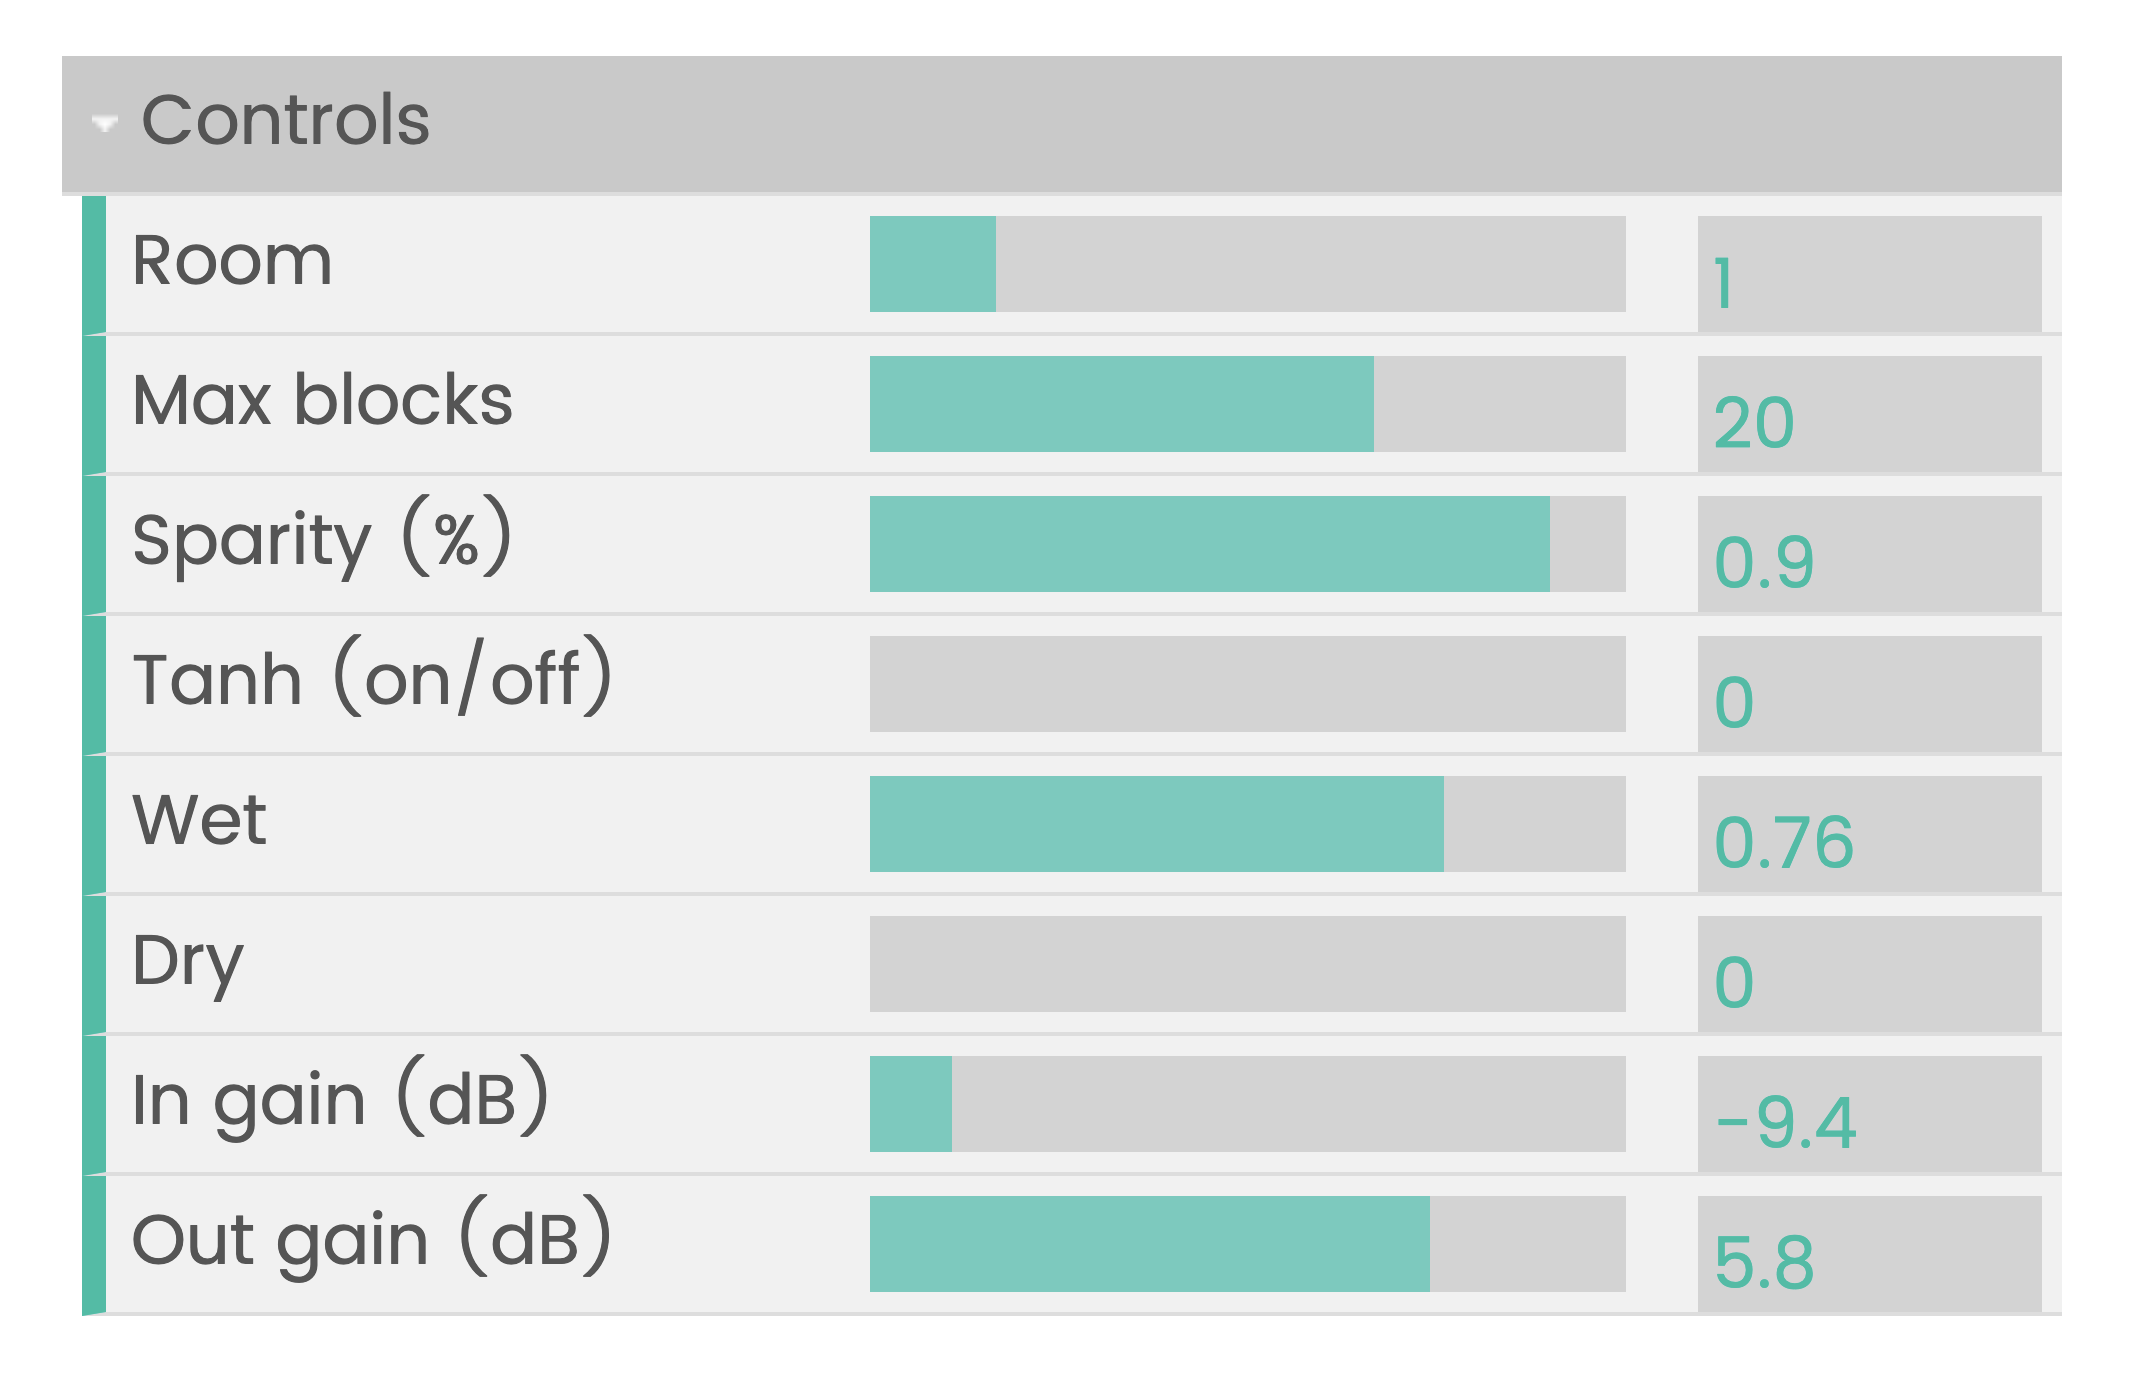
\includegraphics[width=0.6\linewidth]{figures/ui.png}
    \caption{User interface}
    \label{fig:ui}
\end{figure}

A number of sliders are provided in a simplistic UI as shown in Figure~\ref{fig:ui}.
This enables user interaction with the convolution algorithm in real-time. 
The first slider, named \emph{Room} enables the user to switch between six different pre-loaded RIRs. 
These RIRs are sourced from various locations and include a range of rooms, from small, medium, to a large church, as well as plate reverb. 
Setting the \emph{Room} slider to 6 will result in a bypass of the reverb effect. 

The \emph{Max blocks} control adjust the maximum number of blocks of the filter applied. 
As the value is reduced, and blocks at the end of the filter beyond the maximum allowed will be excluded.
This can be utilized as a way to shorten the reverb time, and also reduce the computational load. 

In addition, the \emph{Sparsity} control enables another way to ignore blocks in the convolutional filter. 
Instead of only removing blocks from the end of the filter, this control will progressively remove 
blocks from the across the entire filter. 
While a very low \emph{Sparsity} provides the best sonic results, higher values produce an interesting delay like effect, 
due to the periods of sparsity in the resultant effective filter. 

A simple toggle is provided to activate a tanh nonlinearity.
This is followed by \emph{Wet} and \emph{Dry} mix controls, which are common in most reverb effects. 
Finally \emph{In gain} and \emph{Out gain} controls are provided in order to either push the nonlinearity, 
or reduce the output gain in the case of loud impulse responses. 

\section{Evaluation}\label{sec:eval}

As the first part of the evaluation, the runtime of both the \texttt{DirectConvolver} and \texttt{FFTConvolver} are compared.
To do so, the time required to compute $N$ output samples with a filter of length $N$ was averaged over 100 blocks. 
To eliminate the effect of the block size in the these measurements, a large block size of 4096 samples was used. 
The results are reported in Figure~\ref{fig:runtime}.
This agrees with our intuition, where as the filter size grows the compute time for the direct form implementation increases linearly. 
For the the FFT implementation, the computation time grows significantly slower as the filter size and input size increase.
Looking closely at the results, after the filter size increases beyond 32 samples, the FFT computation becomes more efficient. 
This was then used as the base value for $N$ when setting up the \texttt{ZLConvolver}. 

\begin{figure}[h]
    \centering
    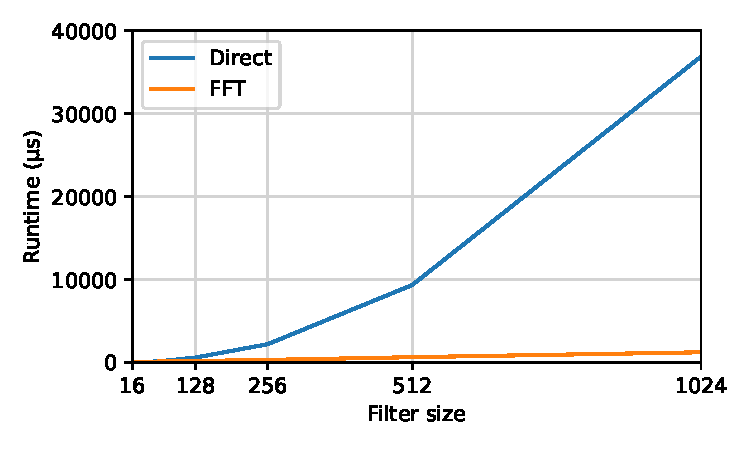
\includegraphics[width=0.65\linewidth]{figures/runtime.pdf}
    \caption{Runtime for filters of size $N$ and input blocks of size $N$.}
    \label{fig:runtime}
\end{figure}

As a more informal evaluation, the ability to operate at different block sizes was investigated. 
Performance is manageable down to a frame size of 8 samples, but underuns occur at a frame size of 4. 
Things function well at frame sizes of both 16 and 32, but utilizing a frame size larger than 32 causes an issue in the current implementation.
This is due to the choice of $N=32$, since when the frame size is 64, all 64 samples must be computed by the end of the period.
Due to the auxiliary tasks that will be computing the following samples, these lower priority tasks will not be completed by the time that 
the main thread reads values from the output buffer and sends them to the audio output. 
Adjusting $N$ to be a larger value does not help this significantly. 
Instead, this would require a way to ensure that FFT convolvers 
on other threads complete their computation for output samples in the 
current frame before the values are read out and sent to the audio output. 

Since one of the other purposes of this work was to investigate the feasibility of implementing a real-time neural audio effects
with the low-latency convolution the ability to run multiple convolutions in series was tested.
Unfortunately, the computational cost of a single convolution on Bela is already quite high, and therefore it was not possible 
to go beyond two medium sized convolutions. This is simply not enough to implement an effective TCN, 
which likely requires at least two layers, with the first layer featuring a multiple channel convolution.  
For that reason, the final design of the program is focused on the simple convolutional reverb, which is fully functional. 

\subsection{Demonstration}

A short demonstration of the convolutional reverb is available online\footnote{\url{https://youtu.be/PuP8an5F2rk}}.
This video demonstrates the basic functionality of the zero-latency convolver on Bela.
First a simple looping guitar riff is used as a source signal, 
which is processed in real-time using a small block size of 16 samples. 
Note that the audio quality is not ideal since sound from Bela is recorded being played over a loudspeaker.
The function of the different controls are presented along with a demonstration of the six different room impulse responses. 
In addition to the guitar signal, a flute recording is also used to demonstrate some of the functionality. 

\subsection{Limitations}
While this implementation was capable of achieving a low-latency convolution on Bela with long convolutional filters up to 3 seconds, 
there are certainly some performance instabilities. 
The CPU usage required by the current implementation is often quite high and on the longest impulses responses 
this can sometimes result in the Bela losing connection to the host, while audio remains playing. 
Additionally, this implementation was not efficient on Bela to enable a multiple channel convolution for emulating a TCN. 

\section{Conclusion}\label{sec:conclusion}

In this project a `zero-latency' convolutional reverb was implemented on the Bela platform.
While it was demonstrated that this implementation was successful in achieving real-time low-latency convolution 
with a large impulse response of over 3 seconds, this required all of the compute resources on Bela. 
Initial experiments to implement a simple temporal convolutional network utilizing this implementation 
were therefore not successful, since it was not feasible to run more than two short convolutions in series.
Nevertheless, the resultant low-latency convolution works well on Bela. 
To demonstrate the potential of this implementation a simple UI was constructed that enables user
to switch through six different room impulse responses and adjust various parameters.
Max blocks and sparsity controls were introduced to both adjust the sound of the the prerecorded impulse responses, 
as well as potentially reduce the computational load of very long impulse responses. 
Future work will consider other potential optimizations mentioned in the literature, 
as well as the investigation of other methods for inducing sparsity in the block-based FFT convolution, 
which may be applicable for implementing low-latency convolution for real-time neural audio effects. 

\cleardoublepage
\bibliographystyle{unsrt}
\bibliography{references}

\end{document}
